% ===============================================================================
\section{Structure detection packages}
Before starting implementing code to enable \wingj to support additional biological systems, a new Java package must be created. This package will later contains all the Java classes and methods that are required to enable the unsupervised structure detection of a given organ or body system. For example, \wingj initially implements an unsupervised structure detection for the \droso wing pouch and a weakly-supervised method for the \droso embryo \autocite{schaffter2013}. Their respective package name is:

%\footnote{\wingj doesn't require the structure detection to be fully automatic and may ask users for interactions depending the the algorithms you will implement. Note that \wingj provides a step-by-step mode to supervise the application of each detection module.}

\begin{itemize}
 \item \wingpouchLongPkg
 \item \embryoLongPkg
\end{itemize}

The name of these two packages follows the Java \javaNamingConventions. These two package names actually correspond to two directories:

\begin{itemize}
 \item ch/epfl/lis/wingj/structure/drosophila/wingpouch
 \item ch/epfl/lis/wingj/structure/drosophila/embryo
\end{itemize}

New packages must be created in the \structurePkg package of \wingj. First, create a folder named after the name of the \textit{organism} of interest (if not already existing). Characters are limited to lowercase letters (a-z) and numbers if required (avoid white spaces ' ' or any other separators). Examples are \textit{drosophila}, \textit{zebrafish}, \textit{yeast}, etc.\\

Inside the \textit{organism} folder, create a second folder named after the name of the \textit{organ} or system you want to study. You should then obtain the following folder structure:

\begin{itemize}
 \item ch/epfl/lis/wingj/structure/\textit{organism}/\textit{organ}
\end{itemize}



% ===============================================================================
\section{\droso wing pouch}\label{sec:wing_pouch_structure_detection}
\subsection{Overview}
Here we explain how to implement a structure detection method using the design of the methods already provided by \wingj. The inference of the \droso wing pouch structure takes as input a single image or a stack of confocal fluorescence images. In the latter case, we compute the maximum intensity projection (MIP) of the stack to obtain a single image where the structure of the pouch is well visible, e.g. by labelling the expression of Wg-Ptc. Here, Wingless (Wg) is used to delimit the outer boundary (or contour) of the wing pouch and the D/V compartment boundary, and the expression of Patch (Ptc) for identifying the A/P compartment boundary. Our method generates a parametric model of the wing pouch structure before inferring its orientation in the image space (A/P and D/V directions). The identity of each compartment DA, DP, VA, and VP is then unravelled. More detailed information about the methods we developed is available in the \textbf{Supplementary Notes} of our paper \autocite{schaffter2013}.

% ===============================================================================
\subsection{Class organization}
\figureref{fig:wpouch_diagram} shows the organization of the classes in the package \wingpouchPkg. A minimum of five abstract classes have to be extended for enabling \wingj to infer a structure model. The abstract classes can be found in the package \structurePkg and provide ``templates'' for implementing the required system-specific classes. An additional class to extend is \WJSystem which will provide the interface between \wingj and the structure detection package of the system (\sectionref{sec:wing_systems}).

% The function of each abstract classes is described in more detail in the next sections.

\begin{figure}[h]
\centering
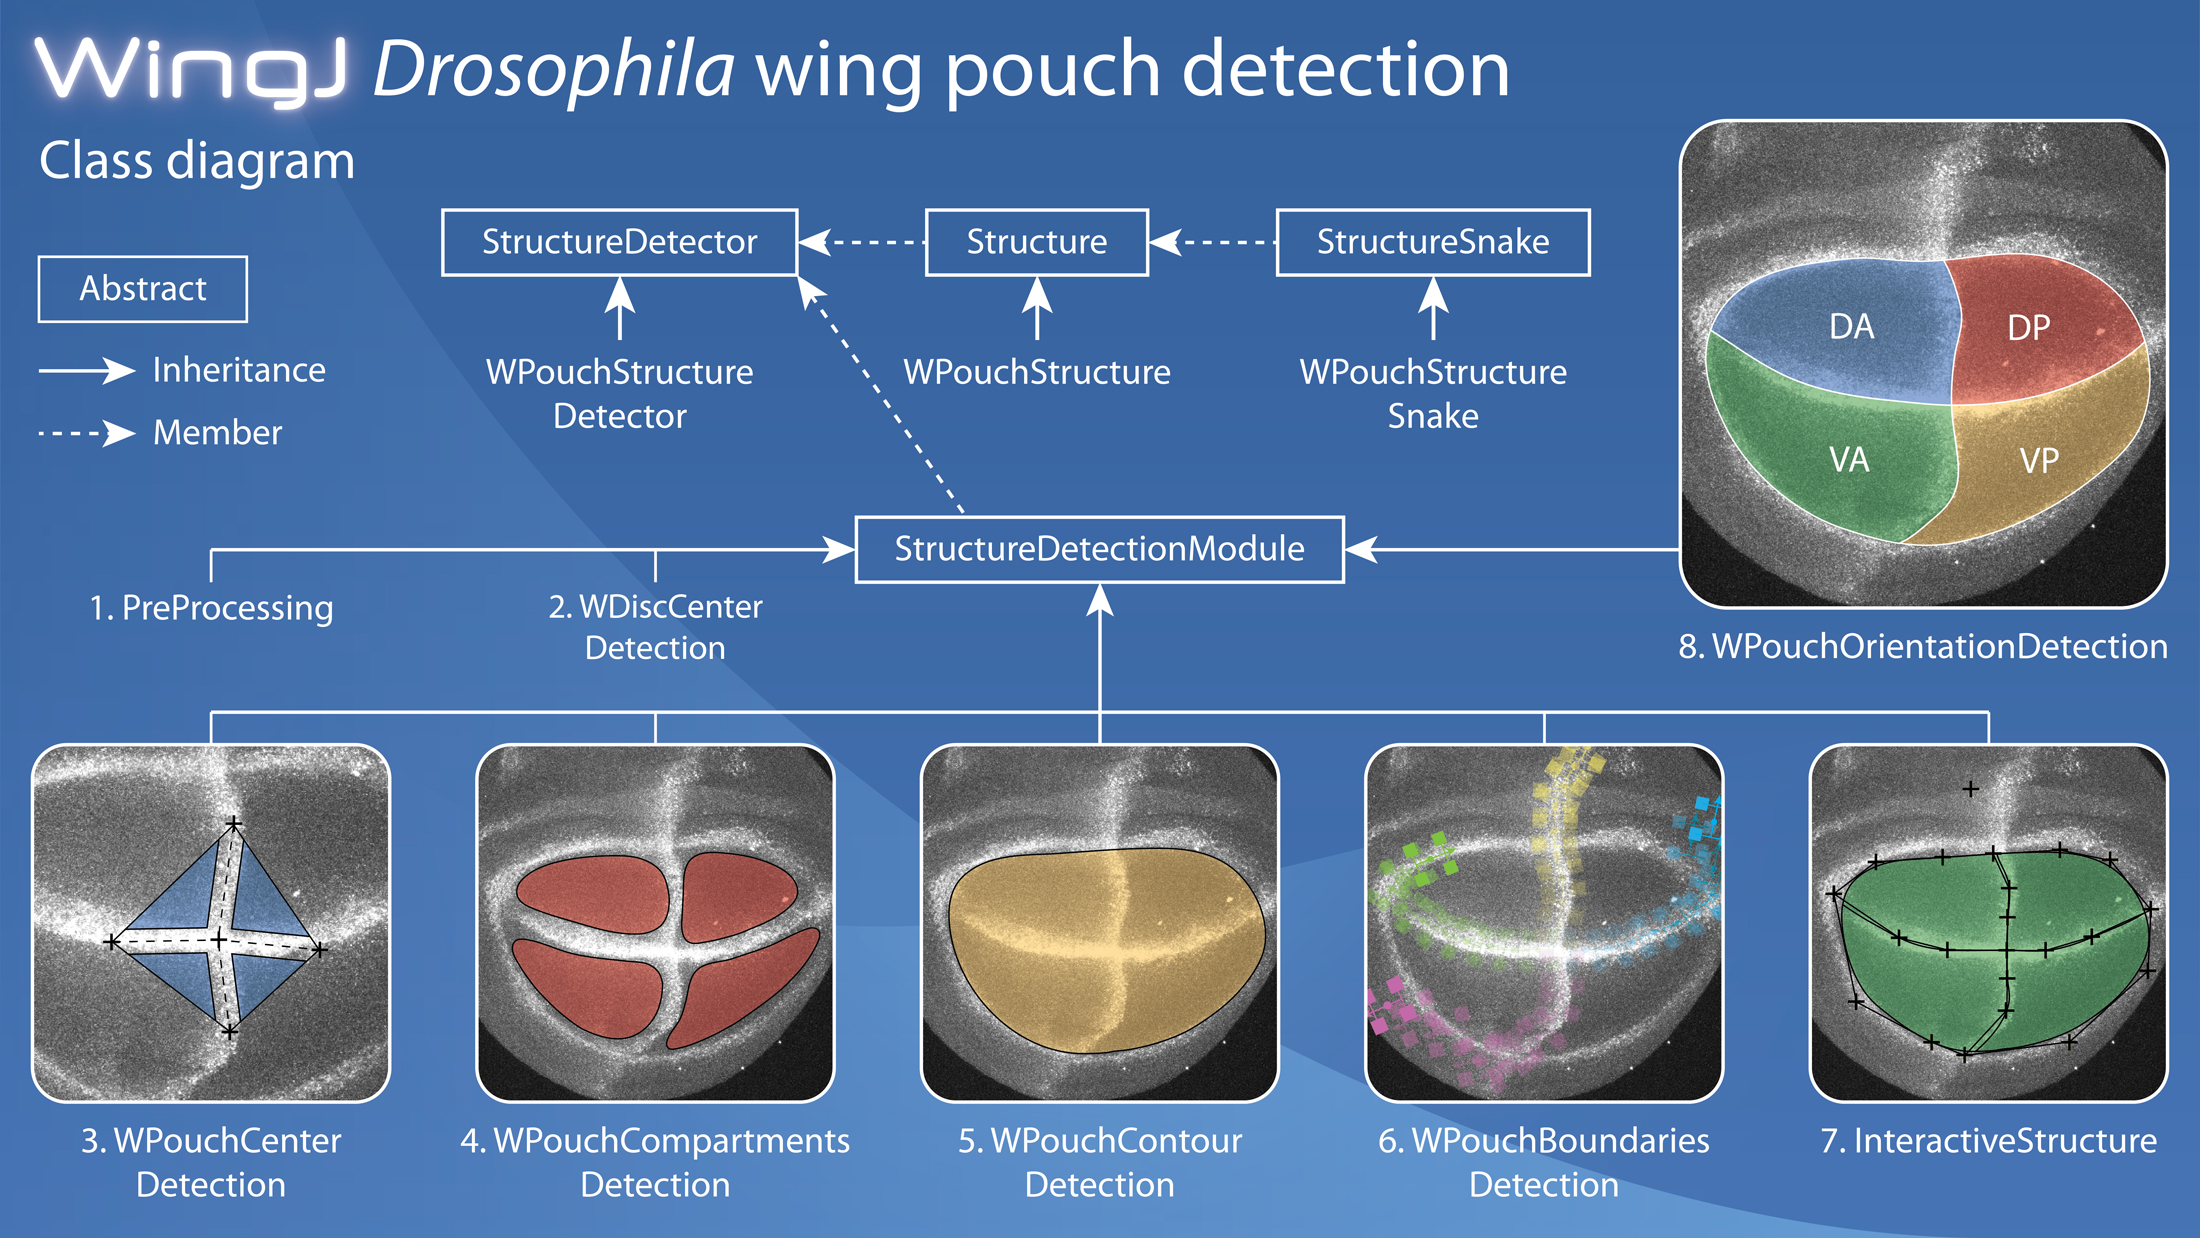
\includegraphics[width=146mm]{images/wingj-wpouch-diagram_300dpi.jpg}
\caption{\textbf{Class diagram of the structure detection method implemented in \wingj for quantifying \droso wings.} The structure detector \WPouchStructureDetector extends the abstract class \StructureDetector which implements methods such as \textit{run()}, \textit{step()} or \textit{pause()} to interact with the structure detection process. The structure detection is performed by several \emph{detection modules} that extend the abstract class \StructureDetectionModule. The task of each detection module is to identify a specific feature of the overall structure to model. Here the outputs of as much as eight detection modules are combined to generate a parametric description (extending \WPouchStructureSnake) of the wing pouch structure. Finally, a \WPouchStructure object is initialized with the data contained in \WPouchStructureSnake to build a model including instances of \Compartment and \Boundary. Furthermore, \WPouchStructure includes information about the A/P and D/V orientation of the structure in the image space.}
\label{fig:wpouch_diagram}
\end{figure}

% Before describing in more detail the function of each abstract class, we list below all the classes included in the package \wingpouchPkg in alphabetical order and give a short description.

% ===============================================================================
\subsection{Structure}
The class \WPouchStructure extends the abstract class \Structure and represents a morphological structure including \Compartment and \Boundary objects. For instance, the wing pouch is divided by the A/P and D/V compartment boundaries into four compartments DA, DP, VA, and VP. \WPouchStructure also contains information about the A/P and D/V orientation of the wing pouch in the image space.

% ===============================================================================
\subsection{StructureSnake}
The class \WPouchStructureSnake extends the abstract class \StructureSnake, which is a member variable of \Structure. \WPouchStructureSnake implements a parametric model of the wing pouch structure using B-splines \autocite{DelgadoGonzalo2012}. The user can interact with the parametric model thanks to the detection module \InteractiveStructure introduced in \sectionref{sec:wpouch_modules}. At that stage of the detection, the user is provided with tools to modify the shape of the structure identified by moving around the control points of its model (if required). After validating the parametric model (\WPouchStructureSnake), \WPouchStructure is set with \Compartment and \Boundary objects before inferring the orientation of the wing pouch in the image space \autocite{schaffter2013}.

% ===============================================================================
\subsection{StructureDetector}
The class \WPouchStructureDetector extends the abstract class \StructureDetector, which implements methods to run structure detections. Examples are the methods \textit{run()} (runs a complete structure detection), \textit{step()} (performs a single step/detection module), \textit{pause()} (pauses the detection) and \textit{resume()} (restarts the detection from where it has been paused). At the end of the detection process, the \Structure object contained in \StructureDetector is set.

% ===============================================================================
\subsection{StructureDetectionModules}\label{sec:wpouch_modules}
The abstract class \StructureDetectionModule provides a template class for implementing different steps or \emph{detection modules} applied during the structure detection. Typically, each module is designed to detect a specific feature of the overall structure to model. This modular approach has several benefits. First, extending \wingj to support additional biological systems can benefit from existing detection modules (e.g. modules to identify closed compartments, to identify the trajectory of fluorescent boundaries, etc.). The fluorescence boundary tracker whose behavior is inspired from line-following robots is used in \WPouchBoundariesDetection and can be applied to identify any trajectory along which fluorescence is expressed. Moreover, each module can be modified or replaced to test novel detection strategies. Finally, the robustness of the overall structure detection could be increased by combining the outputs of multiple modules applied to identify the same feature (so-called \textit{wisdom of the crowd} \autocite{surowiecki2004wisdom}).\\

The list of detection modules we developed to generate a comprehensive model of the wing pouch structure is given below.

\begin{enumerate}
 \item \PreProcessing. Sets a few parameters depending on the intrinsic information contained in the input images.
 \item \WDiscCenterDetection. Detects the center of mass of the wing imaginal disc (required for the automatic inference of the orientation of the wing pouch).
 \item \WPouchCenterDetection. Detects the intersection of the A/P and D/V boundaries. We developed and provide two tools that can be used again for detecting the point of intersection between two fluorescence boundaries, see \PlusShapeCenterDetector and \KiteSnake.
 \item \WPouchCompartmentsDetection. Detects the four compartments included in the wing pouch using active active contour segmentation algorithm. The tool we developed to detect the compartments is called \CompartmentSnake.
 \item \WPouchContourDetection. Detects the contour of the wing pouch by creating a convex hull based on the four compartments detected previously.
 \item \WPouchBoundariesDetection. Detects the trajectory of the A/P and D/V compartment boundaries. The tool we developed to identify a trajectory along which fluorescence is expressed is called \FluorescenceTrajectoryTracker.
 \item \InteractiveStructure. Displays the inferred parametric model of the wing pouch structure on top of the input image(s). The shape of the structure can be modified by moving the control points '+' which correspond to the parameters of the model.
 \item \WPouchOrientationDetection. Infers automatically the orientation of the wing pouch in the image space using prior information about the geometry of the wing pouch structure.
\end{enumerate}

The list of detection modules is defined in \WPouchStructureDetector.\-initialize\-Detection\-Modules() which extends the abstract class \StructureDetector.\-initialize\-Detection\-Modules(). The constructor of a detection module can be provided with the following arguments.

\begin{itemize}
 \item \textbf{String name}. The name and identifier of the detection module.
 \item \textbf{StructureDetector detector}. The reference to the structure detector (instance of \StructureDetector) that uses this module.
 \item \textbf{Boolean hidden}. If set to true, the next module is run automatically once the current detection module is done. If false, the user must click on \textit{Step} or \textit{Resume} to continue. Stopping after the execution of each detection module can be used to allow the user to check/debug the output of the current module.
\end{itemize}

The following portion of code is used in \StructureDetector.step(int i) to run the i\textsuperscript{th} detection module:\\

% \begin{codebox}
\footnotesize\texttt{// ============================================================================\\
// RUNS CURRENT DETECTION MODULE\\
detection.run();\\
while (!detection.test()) \{\\
\indent \ \ \ if (stop\_) // in case detection has been stopped\\
\indent \ \ \ \ \ \ \ return moduleIndex\_;\\
\indent \ \ \ detection.update();\\
\indent \ \ \ ...\\
\indent \ \ \ detection.run();\\
\}}\normalsize\\
% \end{codebox}

Each detection module should override three methods defined in \StructureDetectionModule and listed below. If one of these methods throws an exception, the detection is stopped and a message is shown to the user. After modifying a parameter, for instance, the structure detection can be resumed by pressing on the button \textit{Resume} or \textit{Step}.

\begin{itemize}
 \item \textbf{run()}. Implements the method to identify a specific feature of the overall structure to model.
 \item \textbf{test() (optional)}. Implements multiple tests and returns true if the output is considered as correct. If \emph{test()} is not overridden, \emph{test()} returns true.
 \item \textbf{update() (optional)}. If \emph{test()} returns false, a parameter adjustment can be applied before running once again (and automatically) the method \emph{run()}. \emph{update()} can be used to prompt the user to enter a parameter value or implement an automatic incrementation of a parameter value, for example.
\end{itemize}

Remember that the detection modules have access to the reference of the \WPouchStructureDetector and \WPouchStructure objects. The module \InteractiveStructure is used to display the inferred model and allows users to interact with it. When the model is validated, \WPouchStructureSnake is updated and \WPouchStructure is built. After applying \WPouchOrientationDetection, \WPouchStructure is updated to include information about the orientation of the structure and thus obtain a consistent model of the wing pouch structure.


\clearpage
% ===============================================================================
\section{\droso embryo}
\subsection{Overview}
The implementation of the \droso embryo structure detection is similar to the detection of the wing pouch but requires the design of less detection modules. \figureref{fig:embryo_diagram} shows the organization of the most important classes. The structure detection consists in first identifying the contour of the embryo before defining the A/P and D/V compartment boundaries. In the current implementation, the user is asked to place the free vertex '+' inside the DA (dorsal-anterior) compartment to before inferring automatically the identity of the remaining DP, VA, and VP compartments. That's why the proposed method is weakly-supervised and not unsupervised. One way to fully automate this process could be to use the information provided by a protein whose expression is asymmetrically distributed in the embryo. Such protein could be the \textit{hairy} protein.

\begin{figure}[h]
\centering
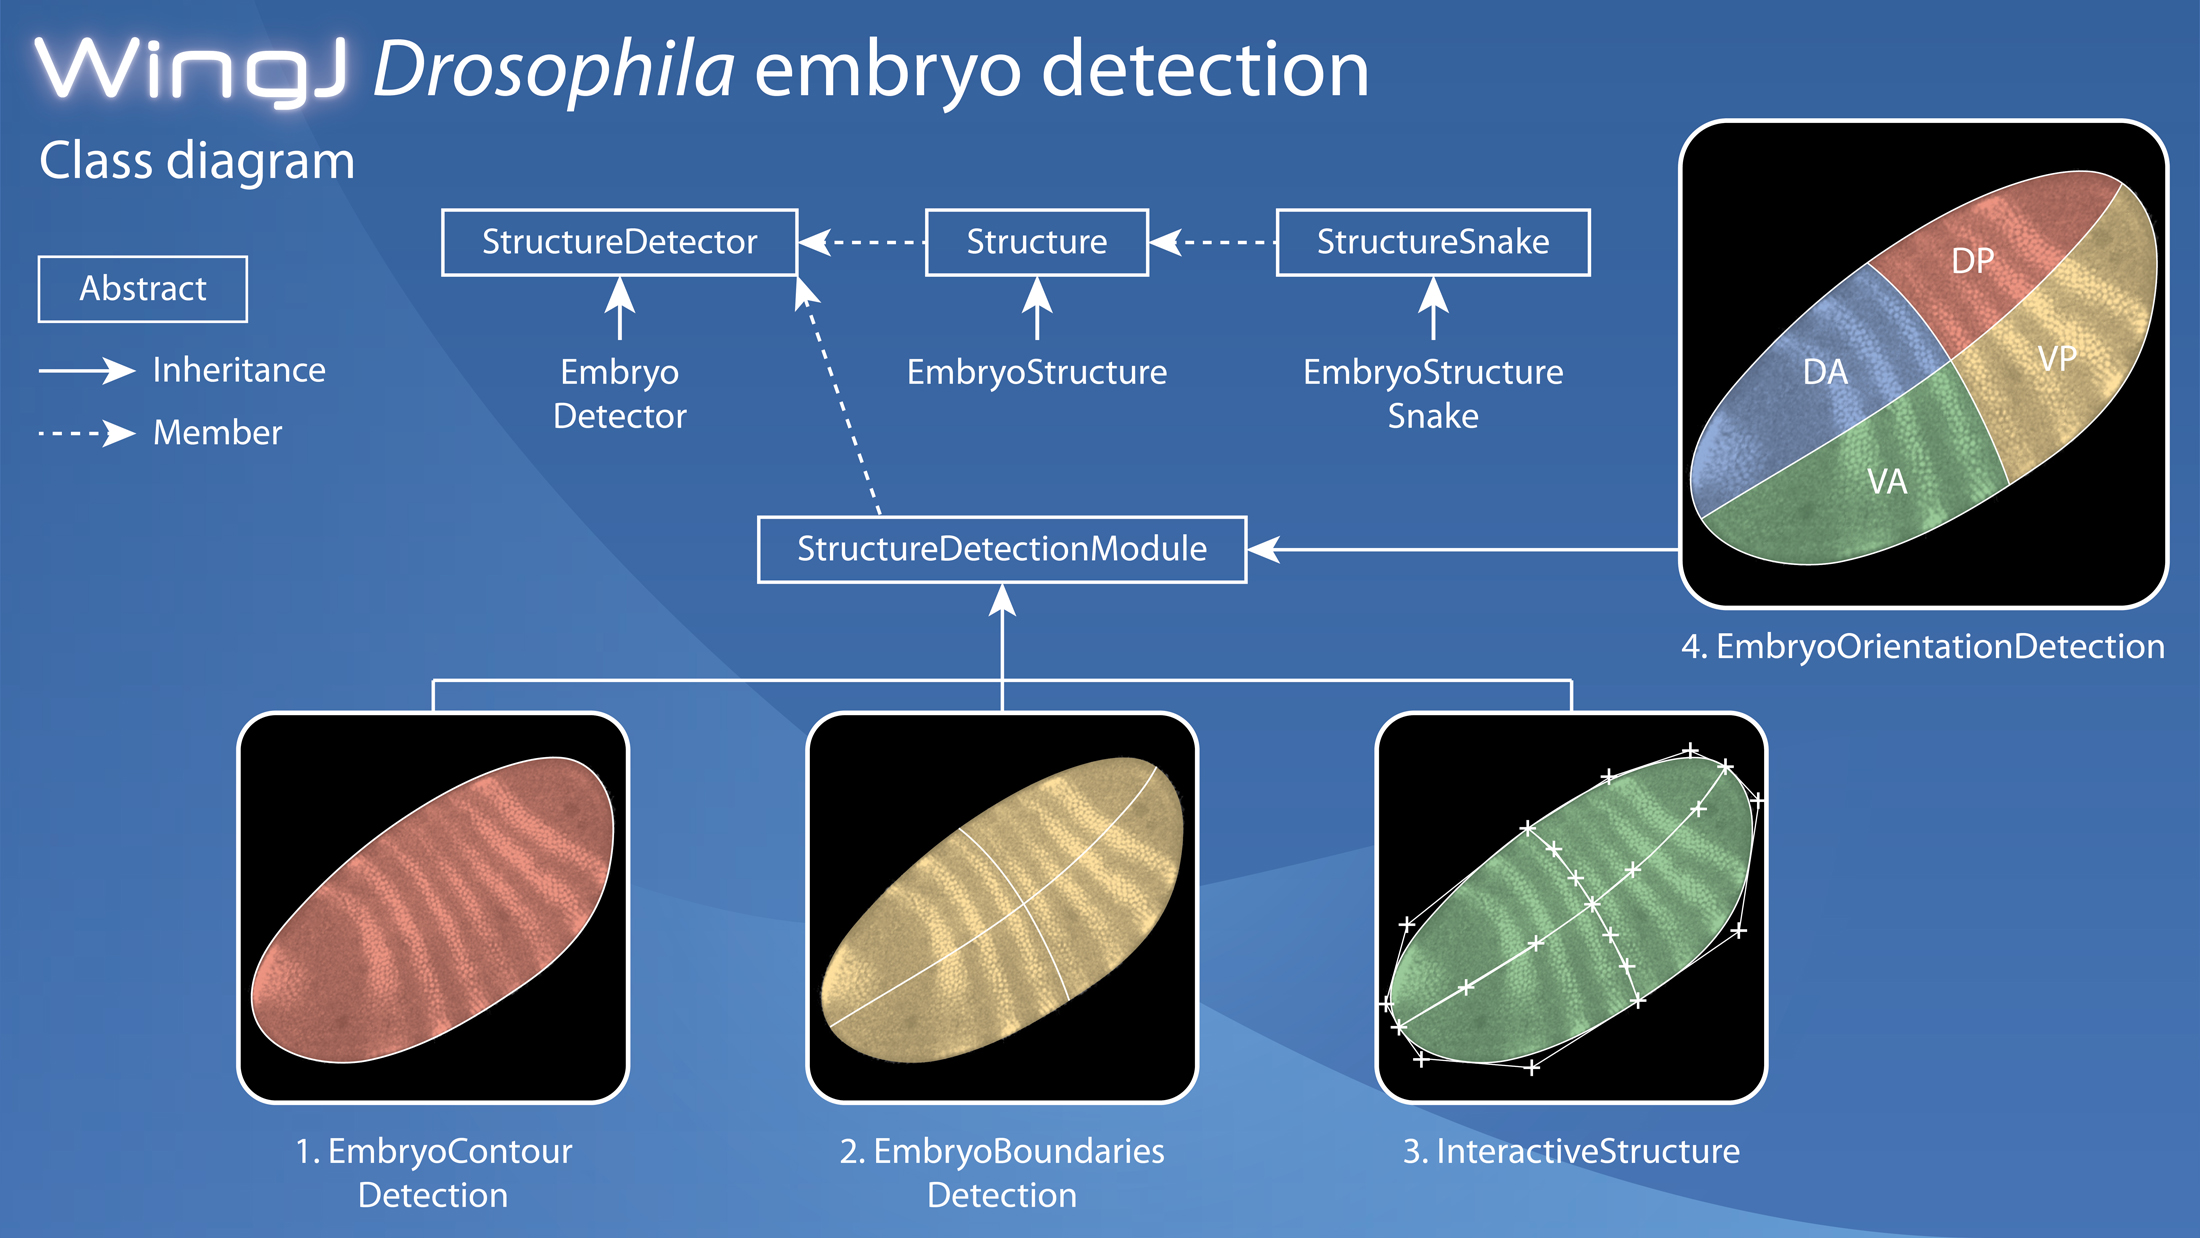
\includegraphics[width=146mm]{images/wingj-embryo-diagram_300dpi.jpg}
\caption{\textbf{Class diagram of the structure detection method implemented in \wingj for quantifying \droso embryos.} The structure detector \EmbryoStructureDetector extends the abstract class \StructureDetector which implements methods such as \textit{run()}, \textit{step()} or \textit{pause()} to interact with the structure detection process. The structure detection is performed by several \emph{detection modules} that extend the abstract class \StructureDetectionModule. The task of each detection module is to identify a specific feature of the overall structure to model. Here the outputs of four detection modules are combined to generate a parametric description (extending \EmbryoStructureSnake) of the embryo structure. Finally, a \EmbryoStructure object is initialized with the data contained in \EmbryoStructureSnake to build a model including instances of \Compartment and \Boundary. Furthermore, \EmbryoStructure includes information about the A/P and D/V orientation of the structure in the image space.}
\label{fig:embryo_diagram}
\end{figure}

% ===============================================================================
\subsection{StructureDetectionModules}

The list of detection modules we developed to generate a model of the \droso embryo structure is given below. Apart from the design of new modules, the overall detection process of the embryo structure is similar to the description given in \sectionref{sec:wing_pouch_structure_detection} for the detection of the \droso wing pouch. The embryo segmentation is much simpler than the detection of the wing pouch as it only requires four detection modules when the wing currently requires eight.

\begin{enumerate}
 \item \EmbryoContourDetection. Detects the contour of the embryo using a snake algorithm.
 \item \EmbryoBoundariesDetection. Defines the A/P and D/V compartment boundaries as the axes of the embryo ellipse shape previously identified.
 \item \EmbryoInteractiveStructure. Displays the embryo structure identified on top of the input image. The shape of the structure can be modified by moving the control points '+' which correspond to the parameters of the structure model.
 \item \EmbryoOrientationDetection. Detects the A/P and D/V orientation of the embryo in the image space from the identity of the DA (dorsal-ventral) compartment given by the user.
\end{enumerate}

% ===============================================================================
\section{WJSystem}\label{sec:wing_systems}
The class \WPouchSystem extends the abstract class \WJSystem, which provides an interface between \wingj and structure detection packages. For example, \wingj creates new structure detectors for the selected system by calling:\\
\emph{WingJ.getInstance().getSystem().newStructureDetector("myExperiment");}\\

One can get the instance of the current structure model using:\\
\emph{WingJ.getInstance().getSystem().getStructureDetector().getStructure();}\\

After creating a new class extending \WJSystem, set its member variables \emph{name\_} and \emph{description\_} (you may have a look at the description of existing systems for examples), and implemented the different abstract methods. Then, register the new system in \WJSystemManager to make it available to \wingj. At startup, \wingj instantiate the different system and list them in a drop-down list on the main interface. The description of the system can be displayed by simply placing the mouse pointer hover this list. A tooltip will then appear with the content of the description previously set. Note that the HTML format can be used to highlight elements in the text, for instance \emph{description\_ = "\textless html\textgreater This word is in \textless i\textgreater italic\textless /i\textgreater.\textless /html\textgreater";}.

% ===============================================================================
\section{Let us know}
Please contact if you have implemented a structure detection method for detecting and segmenting an additional biological system (organ system or body system). This also concerns improved versions of existing detection modules and modules that implement a different approach to achieve even higher performance. We will then integrate them in \wingj and make them available to the community. Please contact us if you have any questions regarding the implementation of \wingj or the different methods we developed.